\textbf{LeVeque 1.2} \\\\
a)  Use the method of undetermined coefficients to set up the $5\times5$ Vandermonde system which would determine a 
  fourth-order accurate finite difference approximation to $u''(x)$ based on five equally spaced points:

  $$
    u''(x) = c_{-2}u(x-2h) + c_{-1}u(x-h) + c_0u(x) + c_1u(x+h) + c_2u(x+2h) + \mathcal{O}(h^4)
  $$


\begin{solution}\ \\\\
    We begin by finding the Taylor expansion about each of our points; because our approximation contains five points,
    we need only determine the first five terms:

    \begin{align*}
    u(\bar{x} - 2h) &= u(\bar{x}) + \frac{(-2h)}{1!}u^{(1)}(\bar{x}) 
                                 + \frac{(-2h)^2}{2!}u^{(2)}(\bar{x}) 
                                 + \frac{(-2h)^3}{3!}u^{(3)}(\bar{x})
                                 + \frac{(-2h)^4}{4!}u^{(4)}(\bar{x})
                                 + \mathcal{O}(h^5) \\
    u(\bar{x} - h) &= u(\bar{x}) + \frac{(-h)}{1!}u^{(1)}(\bar{x}) 
                                 + \frac{(-h)^2}{2!}u^{(2)}(\bar{x}) 
                                 + \frac{(-h)^3}{3!}u^{(3)}(\bar{x})
                                 + \frac{(-h)^4}{4!}u^{(4)}(\bar{x})
                                 + \mathcal{O}(h^5) \\
    u(\bar{x}) &= u(\bar{x}) \\
    u(\bar{x} + h) &= u(\bar{x}) + \frac{(h)}{1!}u^{(1)}(\bar{x}) 
                                 + \frac{(h)^2}{2!}u^{(2)}(\bar{x}) 
                                 + \frac{(h)^3}{3!}u^{(3)}(\bar{x})
                                 + \frac{(h)^4}{4!}u^{(4)}(\bar{x})
                                 + \mathcal{O}(h^5) \\
    u(\bar{x} + 2h) &= u(\bar{x}) + \frac{(2h)}{1!}u^{(1)}(\bar{x}) 
                                 + \frac{(2h)^2}{2!}u^{(2)}(\bar{x}) 
                                 + \frac{(2h)^3}{3!}u^{(3)}(\bar{x})
                                 + \frac{(2h)^4}{4!}u^{(4)}(\bar{x})
                                 + \mathcal{O}(h^5) \\
    \end{align*}

    We now collect coefficients; since we are interested in an an approximation for $u^{(2)}(x)$, each
    collection of coefficients sums to zero save for that of the second derivative:

    \begin{align*}
    \begin{cases}
        c_{-2} + c_{-1} + c_0 + c_1 + c_2 = 0 \\
        (-2h)c_{-2} + (-h)c_{-1} + (h)c_1 + (2h)c_2 = 0 \\
        (2h^2)c_{-2} + (\frac{1}{2}h^2)c_{-1} + (\frac{1}{2}h^2)c_1 + (2h^2)c_2 = 0 \\
        (-\frac{4}{3}h^3)c_{-2} + (-\frac{1}{6}h^3)c_{-1} + (\frac{1}{6}h^3)c_1 + (\frac{4}{3}h^3)c_2 = 0 \\
        (\frac{2}{3}h^4)c_{-2} + (\frac{1}{24}h^4)c_{-1} + (\frac{1}{24}h^4)c_1 + (\frac{2}{3}h^4)c_2 = 0 \\
    \end{cases}
    \end{align*}

    Lastly, we divide each equation by an appropriate power of $h$ and write the result as a $5 \times 5$ linear system, as desired:

    $$
    \begin{pmatrix}
        1            &           1  & 1 &           1 & 1 \\
        -2           &           -1 & 0 &           1 & 2 \\
        2            & \frac{1}{2}  & 0 & \frac{1}{2} & 2 \\
        -\frac{4}{3} & -\frac{1}{6} & 0 & \frac{1}{6} & \frac{4}{3} \\
        \frac{2}{3}  &           -1 & 0 & 1           & \frac{2}{3} \\
    \end{pmatrix}
    \begin{pmatrix}
        c_{-2} \\ c_{-1} \\ c_0 \\ c_1 \\ c_2
    \end{pmatrix}
        =
    \begin{pmatrix}
        0 \\
        0 \\
        \frac{1}{h^2} \\ 
        0 \\
        0 \\
    \end{pmatrix}
    $$
\end{solution}


b)  Compute the coefficients using the MATLAB code \texttt{fdstencil.m} available from the website, and check that they
  satisfy the system determined in part (a).



\begin{solution}\ \\\\

    Executing \texttt{fdstencil(2, -2:2)} yields the following output: \\\\

    \begin{lstlisting}[language=bash]
octave:1> fdstencil(2, -2:2)
 
The derivative u^(2) of u at x0 is approximated by
 
          1/h^2 * [
                     -8.333333333333333e-02 * u(x0-2*h) + 
                      1.333333333333333e+00 * u(x0-1*h) + 
                     -2.500000000000000e+00 * u(x0) + 
                      1.333333333333333e+00 * u(x0+1*h) + 
                     -8.333333333333333e-02 * u(x0+2*h) ]   
 
For smooth u,
       Error = 0 * h^3*u^(5) + -0.0111111 * h^4*u^(6) + ...
    \end{lstlisting}

    Our coefficients from (a) are therefore:

    \begin{align*}
        \begin{pmatrix}
            c_{-2} \\ c_{-1} \\ c_0 \\ c_1 \\ c_2
        \end{pmatrix}
            = \frac{1}{h^2}
        \begin{pmatrix}
            -\frac{1}{12} \\
            \frac{4}{3} \\
            -\frac{5}{2} \\ 
            \frac{4}{3} \\
            -\frac{1}{12} \\
        \end{pmatrix}
    \end{align*}

    Substituting these coefficients into the $5 \times 5$ Vandermonde system from (a) yields:

    $$
    \frac{1}{h^2}
    \begin{pmatrix}
        1            &           1  & 1 &           1 & 1 \\
        -2           &           -1 & 0 &           1 & 2 \\
        2            & \frac{1}{2}  & 0 & \frac{1}{2} & 2 \\
        -\frac{4}{3} & -\frac{1}{6} & 0 & \frac{1}{6} & \frac{4}{3} \\
        \frac{2}{3}  &           -1 & 0 & 1           & \frac{2}{3} \\
    \end{pmatrix}
    \begin{pmatrix}
        -\frac{1}{12} \\
        \frac{4}{3} \\
        -\frac{5}{2} \\ 
        \frac{4}{3} \\
        -\frac{1}{12} \\
    \end{pmatrix}
        =
    \frac{1}{h^2}
    \begin{pmatrix}
        0 \\
        0 \\
        1 \\
        0 \\
        0 \\
    \end{pmatrix}
        =
    \begin{pmatrix}
        0 \\
        0 \\
        \frac{1}{h^2} \\
        0 \\
        0 \\
    \end{pmatrix}
    $$

    ...which satisfies the system from (a), as desired.

\end{solution}
\pagebreak

c)  Test this finite difference formula to approximate $u''(1)$ for $u(x) = \sin(2x)$ with values of $h$ from the array 
  \texttt{hvals = logspace(-1, -4, 13)}. Make a table of the error vs.\ $h$ for several values of $h$ and compare 
  against the predicted error from the leading term of the expression printed by \texttt{fdstencil}. You may want to 
  look at the m-file \texttt{chap1example1.m} for guidance on how to make such a table.

  Also produce a log-log plot of the absolute value of the error vs.~$h$.  

  You should observe the predicted accuracy for larger values of $h$. For smaller values, numerical cancellation in 
  computing the linear combination of $u$ values impacts the accuracy observed.
    
\begin{solution}\ \\\\
    We denote fourth-order approximation of the second derivative of $u$ at $\bar{x} = 1$ in the table below by
    \texttt{DD4u}. The MATLAB code to produce this table and associated plot are provided in the included 
    \verb|problem_2.m| file. Observe that the error predicted by the leading term of the expression printed by 
    \texttt{fdstencil} matches the actual error quite closely for $h \ge 0.01$: \\

    \begin{lstlisting}[language=bash]
       h           Error [DD4u]    Predicted Error [DD4u]
   1.0000e-01      6.4431e-05      6.4661e-05
   5.6234e-02      6.4588e-06      6.4661e-06
   3.1623e-02      6.4638e-07      6.4661e-07
   1.7783e-02      6.4653e-08      6.4661e-08
   1.0000e-02      6.4608e-09      6.4661e-09
   5.6234e-03      6.3753e-10      6.4661e-10
   3.1623e-03      5.2040e-11      6.4661e-11
   1.7783e-03     -3.9182e-11      6.4661e-12
   1.0000e-03     -2.8103e-10      6.4661e-13
   5.6234e-04     -4.8242e-10      6.4661e-14
   3.1623e-04     -4.3333e-09      6.4661e-15
   1.7783e-04     -9.9178e-09      6.4661e-16
   1.0000e-04     -3.3754e-08      6.4661e-17
    \end{lstlisting}

    \pagebreak

    As expected, we see that the accuracy varies when $h < 0.01$ due to numerical cancellation in computing the linear
    combination of $u$ values, but is log-linear otherwise:

    \begin{figure}[h]
        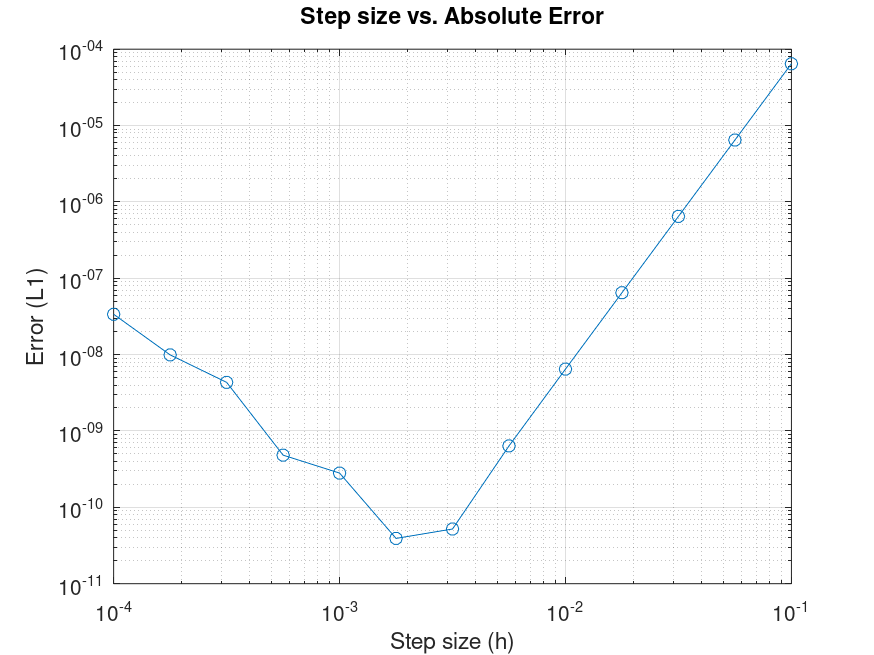
\includegraphics[width=10cm]{fourth-order-uxx-error.png}
        \centering
        \caption{Fourth-order approximation error of second derivative of $\sin{1}$}
    \end{figure}
\end{solution}